\documentclass[11pt]{article}
\usepackage[T1]{fontenc}	%special characters
\usepackage[utf8]{inputenc}	%special characters
\usepackage{lmodern,textcomp}% Euro Symbol

\usepackage{hyperref}
\usepackage[margin=1in]{geometry} %article layout margins
\usepackage{tabularx}		%tabulars width fixed textwidth
\usepackage{multicol}	%2 columns in Skills
\usepackage{graphicx}
\usepackage{sectsty}
\sectionfont{
	\sectionrule{0pt}{0pt}{-5pt}{0.8pt}
}

\begin{document}

\Large
\noindent
\textbf{Dirk Hornung, Ph.D.} \\

\normalsize
\noindent
\begin{minipage}{0.5\linewidth}
  \begin{tabularx}{0.6\textwidth}{>{\bfseries}l l}
    City:           & Barcelona \\
    Date of birth:  & October 5, 1991\\
    Place of birth: & Fulda, Germany \\
    Mobile:         & +34 695460404 \\
    E-mail:         & hello@drdirk.io \\
    Website:      	& drdirk.io
  \end{tabularx}
\end{minipage}
\begin{minipage}{0.5\linewidth}
  \begin{flushright}
    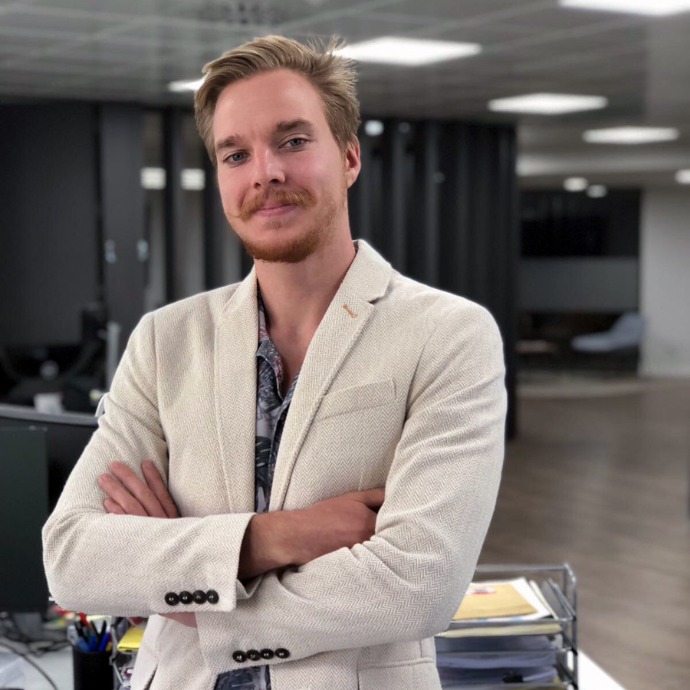
\includegraphics[width=0.4\textwidth]{dirk.png}
  \end{flushright}
\end{minipage}

% Cover Letter
% ------------------------------------------------------------------------------
% \section*{}
% \vspace{1cm}
% Dear Boston Consulting Group, \\

% \noindent I am Dirk Hornung, a recently graduated PhD student at the institute
% of high energy physics of the autonomous university of Barcelona with 5+ years
% of experience in leading the technology in different Startups. Within my
% studies, I researched low-energy QCD and the determination of Standard Model
% parameters. In principle, I found intelligent ways to extract parameters of
% theoretical models out of experimental data. \\

% \noindent Besides my studies, I am an entrepreneur. During the last year, I
% developed Smart Contracts in the Ethereum Blockchain and connected them through
% REST APIs using Node Express for a legaltech. Before I developed a chatbot using
% artificial intelligence for a fintech. We connected our clients through
% Messenger to their bank accounts and analysed their banking information using
% Python. I am furthermore a Full-stack developer with lots of experience
% developing
% applications using React as frontend and AWS services as a backend.  \\

% \noindent In my free time, I prototype IoT devices. I 3D model home security
% devices within Fusion 360, before choosing, connecting and programming the
% electronic circuits. Then I 3D print the necessary parts and
% mount the finished product. \\

% \noindent I am recently graduated and indecisive if creating a company or
% joining a consulting company for further developing my career is the
% better choice. Unlimited 2019 would give me the insights to further plan my future and (possibly) the chance to meet new challenges. \\

% \noindent Sincerely, \\
% Dr Dirk Hornung \\

% \noindent P.S. I am a native German, but also fluent in English, French and
% Spanish. Visit drdirk.io to get to know me better.
% \newpage
% ------------------------------------------------------------------------------

	
% \section*{Professional Profile}
% Theoretical solid-state and high-energy physicist. \hfill 7+ years \\[1mm]
% Data Scientist \hfill 4+ years \\[1mm]
% Software Architect \hfill 2+ years \\[1mm]
% Blockchain Developer \hfill 2+ years \\[1mm]
% Full Stack Developer \hfill 10+ years \\[1mm]

\section*{Professional Experience}
\begin{tabularx}{\textwidth}{lX}
  since July 2019        & \textbf{AI / ML} \\
                         & Absolved the Deep Learning and Machine Learning
                           specialisation on Coursera. Applying Neural Networks to active noise
                           canceling simulations. Creating Recommendation systems.  \\\\
  May 2018 - Jan. 2019   & \textbf{CYSAE} \\
                         & \textit{CTO} (2 Developers) \\[2mm]
                         & \textbf{Utility Token for Cuatre Casas} \\
                         & Customised an ERC-20 Solidity Smart Contract for
                           a Spanish lawyer agency. Configured and launched an
                           Ethereum Node connected to a Node-Express REST API to consume
                           the token functionality. \\[1.5mm]
                         & \textbf{Stamper} \\
                         & Developed a React-Redux Web App with an
                           GraphQL-Prisma-MySQL backend hosted on AWS-ERC docker
                           containers and AWS-S3. \\[1.5mm]
                         & \textbf{Boardchain} \\
                         & Developed a DAO to decentralise board meetings. The
                           Web App was based on React-Redux backed by
                           Serverless AWS-Lambda, AWS-S3, AWS-Cognito and AWS-Dynamodb. \\\\
  Oct. 2017 - Apr. 2018  & \textbf{Alda} \\
                         & \textit{CTO \& Co-Founder} (1 Developer) \\[2mm]
                         & \textbf{Alda Chatbot} \\
                         & Created a Messenger Fintech Chatbot. Modelled and
                           trained a RNN before switching to the Dialogflow API
                           for the NLP. Created a Serverless Python-Flask-AWS-RDS (PostgreSQL) backend,
                           combining the Facebook and Saltedge API to connect
                           and query financial information of our clients. \\[1.5mm]
                         & \textbf{Chatbot UI} \\
                         & Created React-Redux PWA connected to our chatbot.
                           Integrated the app in various Wordpress and Liferay
                           installations. \\\\
  Feb. 2017 - Sept. 2017 & \textbf{WeGoLoco} \\
                         & \textit{CTO \& Co-Founder} \\[1mm]
                         & Created a native iOS app based on Swift. \\

  %                          2017 & \textbf{FuldaCity} \\
  %                          & \textit{CTO \& Co-Founder} \\[1mm]
  %                          & Bringing my Hometown online within the
  %                          Meteor/React Framework \\[1mm]
  %                          & http://www.fuldacity.de/ \\\\
  
  %              %                          \pagebreak
  
  
  
  %                          2013 - 2016 & \textbf{Fulda Strategy Group GbR -
  %                          Management Consultancy} \\
  %                          & \textit{Founder and Managing Director} \\[1mm]
  %                          & Projects in the area of ERP selection and
  %                          implementation, process management and software
  %                          development \\[1mm]
  %                          & www.fulda-strategy.com \\\\
  
  %                          2010 - present & \textbf{Eevents Fulda GbR -
  %                          Event Management} \\
  %                          & \textit{Founder} \\[1mm]
  %                          & Organising of company events, weddings and
  %                          birthdays \\[1mm]
  %                          & www.eevents-fulda.de \\\\
  
  %                          2010 - 2014 & \textbf{Hornung Webdesign -
  %                          Webdesign Agency} \\
  %                          & \textit{Founder} \\[1mm]
  %                          & Developing and maintaining of CMS and SaaS.
  %                          \\\\
\end{tabularx}


\section*{Education}
\begin{tabularx}{\textwidth}{lX}
  2019         & \textbf{Deep Learning Specialisation} \\
               & Absolved five classes of the Coursera specialisation of Deep Learning to study Neural Networks,
                 Hyperparameter tuning, Machine Learning projects, Convolutional Neural Networks and Sequence Models. \\\\
  2015 - 2019  & \textbf{Ph.D., Theoretical Physics}, Autonomous University of
                 Barcelona (Spain) \\
               & Thesis: The QCD Strong Coupling from Hadronic Tau
                 Decays \\
               & Supervisor: Dr. Matthias Jamin \\
               & Created a numerical chi-squared fitting routine, written in
                 C++ using the frameworks BOOST and ROOT. \\\\
  2014 - 2015  & \textbf{M.Sc., Particle Physics}, Autonomous University of
                                Barcelona (Spain) \\
               & Thesis: 1-Loop Anomalous Dimensions of 4-Quark
                 Operators \\
               & Supervisor: Dr. Matthias Jamin \\\\
  2011 - 2014  & \textbf{B.Sc., Condensed Matter Physics}, Goethe University Frankfurt (Germany) \\
               & Thesis: Band Structure Studies of Graphene and Modified
                 Graphene Structure \\
               & Supervisor: Prof. Dr. Roser Valentí
\end{tabularx}
		
\section*{Skills}
\begin{tabularx}{\textwidth}{lX}
  \textbf{Data Science} & Python, Tensorflow, Keras, Pandas, Numpy, Matplotlib, Tensorflow, SVM,
                          NN, CNN, RNN
                          Mathematica \\
  \textbf{Frontend}     & JavaScript, React, React Native, Redux, Flutter, CSS, HTML  \\
  \textbf{Backend}      & AWS, Node, Express, MySQL, PostgreSQL, Node, DynamoDB,
                          Serverless, Flask, Zappa, Django \\
  \textbf{Blockchain}   & Ethereum, Solidity, Smart Contracts, Tokens economy,
                          Decentralised Identity, ICOs \\
  \textbf{Prototyping}  & Arduino, C++, Fusion 360, 3D-Printing, CNC, Electronics \\
  \textbf{Marketing}    & Photoshop, Illustrator, Final Cut Pro, SEO, SEM, Wordpress, PHP \\
  \textbf{Soft}         & Leadership, Public Speaking, Motivating, Mentoring, Confidence, Energy
\end{tabularx}

\section*{Awards}
\begin{tabularx}{\textwidth}{lX}
  June 2019      & \textbf{Imagine Silicon Valley Finalist}. \\
                 &  One of ten finalists of more than 500 applicants who sent in a one minute
                   video (https://www.youtube.com/watch?v=Om1DGAa7Cgw) to be sponsored for a Silicon Valley trip. \\\\
  February 2018  & \textbf{Winner: Imagine Developer Dreamer}. \\
                 &  Got selected to participate in the "Imagine-Express-Train". \\\\
  September 2018 & \textbf{Best Fintech Pitch} \\
                 & Awarded 1st price at Fintech Stage's event ``Fintech War'' of over
                   +16 fintech startups plus a 1k€ cash price \\\\
  July 2018      & \textbf{Winner Adidas Finals Herzogen-Aurach} \\
                 &  Created the ``Adidasum'' ICO for an API data marketplace to
                   democratise data and connect data provider, data scientists and
                   data consumer.\\\\
  May 2018       & \textbf{MetLife Iberia Financial Inclusion Award} \\
                 & Awarded a 4K€ cash price at MetLife Iberia to keep
                   promoting Financial Inclusion. \\\\
  April 2018     & \textbf{Winner Adidas Hackathon Barcelona} \\
                 & Created a system that could uniquely identify faces and track
                   emotions. We trained a model to predict the probability of a
                   client purchasing a certain item in an Adidas store.
\end{tabularx}
		


% \section*{Funding}
% \begin{tabularx}{\textwidth}{sX}
%  2015 - present & Ph.D. PIF grant at the Autònoma de Barcelona (Spain), 1200
	% \euro / month
	% \end{tabularx}


	% \section*{Teaching Experience}
	% 	\begin{tabularx}{\textwidth}{sX}
	% 		2015 - 2018 & Universitat Autònoma de Barcelona, Theoretical Mechanics/
  %   Quantum Mechanics I/ Quantum Mechanics II, Complex Numbers/
  %   Teaching Assistant (Spanish) \\[1mm]
	% 		\centering{2014} & Goethe Universität Frankfurt, Quantum Mechanics I , exercise tutor \\
	% 		& Goethe Universität Frankfurt, Math for Physicists II, exercise tutor \\[1mm]
	% 		2013 - 2014 & Goethe Universität Frankfurt, Math for Physicists I, exercise tutor
	% 		% 	% \end{tabularx}


	% \section*{Publications}
	% 	\begin{tabularx}{\textwidth}{sX}
	% 		2015 & Diogo Boito, \textbf{Dirk Hornung}, Matthias Jamin \\[1mm]
	% 		& "Anomalous dimensions of four-quark operators and renormalon structure of mesonic two-point correlators" \\[2mm]
	% 		&  \textit{arXiv:1510.03812 [hep-ph]}	
	% 	\end{tabularx}


	% \section*{Oral presentations}
	% 	\begin{tabularx}{\textwidth}{sX}
  %    2018 & Aix Marseille Université, ``Determination of the QCD Coupling
  %    from
  %    ALEPH $\tau$-Decay data''
	% 	\end{tabularx}\vspace{1mm}
	% 	\begin{tabularx}{\textwidth}{sX}
	% 	2015 & Universitat Autònoma de Barcelona, Master Thesis Defence of : \\ & ``1-Loop anomalous dimensions of 4-quark operators''
	% 	\end{tabularx}\vspace{1mm}
	% 	\begin{tabularx}{\textwidth}{sX}
	% 		2014 & Goethe Universität Frankfurt, Group Seminar Talk: ``Band structure studies of Graphene and modified Graphene structures''
	% 	\end{tabularx}

	\section*{Languages}
	\begin{tabularx}{\textwidth}{lX}
		German: & native \\
		English: & proficient \\
		Spanish: & proficient \\
		French: & intermediate \\
		Hungarian: & basics 
	\end{tabularx}
	

%  \section*{References}
%	\begin{tabularx}{0.5\textwidth}{@{}l}
%		Prof. Dr. Roser Valentí \\
%		valenti@itp.uni-frankfurt.de \\
%		+49 69 798 47816 \\
%		Institut für Theoretische Physik \\
% 		Goethe-Universität Frankfurt am Main \\
% 		Max-von-Laue-Strasse 1 \\
%		60438 Frankfurt am Main \\
%		Germany 	
%	\end{tabularx}
%	\begin{tabularx}{0.5\textwidth}{ll}
%		Prof. Dr. Matthias Jamin \\
%		jamin@ifae.es \\
%		Institut de Fisica d'Altes Energies (IFAE) \\
%                Universitat Autònoma de Barcelona \\
%                Plaça Cívica \\
%                08193 Cerdanyola \\
%		Spain \\
%		\\
%	\end{tabularx}
	

\end{document}

% LocalWords:  io lX textwidth tabulars sX Adidasum Ph PIF renormalon ph save
% LocalWords:  für Theoretische Physik von Strasse Fisica d'Altes Plaça Cívica
% LocalWords:  Cerdanyola LocalWords
